\chapter{IETF Standards}
\label{Standards}


\section{Adaptation 6LoWPAN}
\label{Intr:6LoWPAN}

%\begin{figure}[htbp]
%  \begin{center}
%    \leavevmode
    %\framebox{
%      \includegraphics[scale=0.6]
%      {/home/bo/Documents/Miniproject/Pics/6LoWPANArc.pdf}%}
%    \caption{6LoWPAN system architecture}
%    \label{fig:6LoWArc}
%  \end{center}
%\end{figure}
%\index{figure 1.2}

6LoWPAN stands for IPv6 over LoWPAN. A LoWPAN is the collection of 6LoWPAN nodes which share a common IPv6 prefix (the first 64 bits of the IP address)~\cite{ShelbyBormann2009}. 6LoWPAN allows for IPv6 packets to be transmitted or received by the IEEE 802.15.4 network. A 6LoWPAN network not only fulfils the requirements of WPAN, but also communicates directly with other IP based networks and nodes without intermediate entities. More advantages of using IPv6 over LoWPAN include (but are not limited to):  
\begin{itemize}
\item IP networks are ubiquitous and pervasive in the current society.  This allows for a use of already completed infrastructures, thus saving time, money and R\&D on building new communication platforms. 
\item Technologies which use IP are thoroughly researched and known to be safe and reliable.  This saves much effort which would need to be spent in testing and debugging new networking technologies. 
\item Another reason why IP technologies might prove more suitable are because much of the intellectual rights held by companies in this field are easily traded and used by many players in the field, as opposed to potential lawsuits and legal hassle which might arise due to large-scale usage of new technologies whose intellectual property rights might not be as transparent as the current IP based ones.
\end{itemize}

Figure~\ref{fig:6LoWArc} gives the system architecture of a simple 6LoWPAN\@. Compared with  Figure~\ref{fig:WSNArc}, a 6LoWPAN network uses a LoWPAN border router (LBR) instead of a gateway  to connect  the WSN to the Internet. This kind of network layer router is much more efficient and easier to design than a protocol translating gateway as it eliminates the need for superfluous translations between potentially large number of protocols, which impairs the entire system's usability and usefulness. Furthermore, the 6LoWPAN network can be connected to any other IP based device, giving it extreme adaptability and flexibility unmatched in traditional gateway systems. 
\newline

The following subsections will give a brief introduction of IPv6, then summarize the main difficulties in combining IPv6 with 802.15.4, and present some solutions which are given by IETF~\cite{RFC4944}. 

\subsection{IPv6}
\label{Intro:6LoW:IPv6}
Being the most accepted network layer protocol, the IP protocol mainly features a universal narrow waist which hides the underlying link technology from the upper layer applications. The traditional IPv4 provides for at most %$2^3^2$ addresses. However, judging by the speed of Internet growth, it was predicted that all IP address would soon be exhausted. On July 25, 1994, the IETF proposed IPv6 with $2^1^2^8$ addresses to be the next generation protocol~\cite{RFC1752}.
\newline

As mentioned in Section~\ref{Intr:IEEE}, the maximum PSDU size that the PHY layer  is able to receive is 127 octets. In the worst-case scenario, this will leave only 81 octets for the MAC layer frame. Meanwhile, IPv6 takes at least 1280 octets as its maximum transmission unit (MTU)~\cite{RFC4919}. How to fit this 1280 octets IP datagram into a much smaller MAC frame was one of the big concerns in realizing 6LoWPAN. The solution to this problem is proposed in~\cite{RFC4944} and will be presented in the following subsection.

\subsection{The Adaptation Layer}
\label{Intr:6LoW:Protocol}
%\index{figure 1.2}
The protocol stack model of a typical 6LoWPAN node proposed by IETF is shown in Figure~\ref{fig:Protocol}.  An adaptation layer, namely 6LoWPAN layer, is specially designed for integrating IPv6 with 802.15.4. In this adaptation layer, IPv6 header compression and data fragmentation will be performed to solve the problem of frame size incompatibility, and along with layer-two forwarding~\texttt{mesh-under}, it would allow IPv6 packets to be transmitted via the 802.15.4 network. The basic 6LoWPAN frame structure is shown in Figure~\ref{fig:Frame}. 
\newline

The first scheme performed is IPv6 header compression. The idea is to eliminate the
header which contains the shared information of the same 6LoWPAN network. 
%\vspace{10pt}
%\begin{figure}[htbp]
%  \begin{center}
%    \leavevmode
    %\framebox{%
%      \includegraphics[scale=0.3]
%      {/home/bo/Documents/Miniproject/Pics/Protocol.pdf}%}
%    \caption{6LoWPAN protocol stack}
%    \label{fig:Protocol}
%  \end{center}
%\end{figure}

%\vspace{-20pt}
%\begin{figure}[htbp]
%  \begin{center}
%    \leavevmode
    %\framebox{
%      \includegraphics
%      {/home/bo/Documents/Miniproject/Pics/Frame.pdf}%}
%    \caption{The basic 6LoWPAN frame structure}
%    \label{fig:Frame}
%  \end{center}
%\end{figure}
% \index{figure 1.2}
That is precisely the reason why it was called the stateless header compression. There are two compression formats: header compression one (HC1) and header compression two (HC2). HC1 and HC2 are respectively responsible for the IPv6 header and transport protocol header.  First, the HC1 reduces the 40 octets IPv6 overhead into 2 octets (1 octet for the HC1 encoding and 1 octet for the hop limit). The HC2 is then used to compress any overhead brought by transport layer protocols such as, for example, UDP, TCP, or ICMP.
\newline



In front of the compressed IPv6 header there is a fragmentation header (Figure~\ref{fig:Frame}). This fragmentation header is only introduced when an IPv6 payload does not fit into a single IEEE 802.15.4 frame;
the payload then needs to be fragmented into several packets. It is used in order to indicate the proper order of the sequences. Figure~\ref{fig:Fragmentation_1} gives the header format for the first
fragment; the header format for subsequent fragments is given in Figure~\ref{fig:Fragmentation_2}.
\newline

When using the routing mechanism~\texttt{mesh-under} (in contrast to~\texttt{route-over}, which forwards packets using IP layer addresses), a mesh addressing header precedes the fragmentation header. Because the source and destination addresses in IPv6 headers are compressed in header compression, this mesh addressing header is needed for packets to be correctly forwarded in a layer-two fashion. The mesh addressing header format with short 16-bit link layer addresses is shown in Figure~\ref{fig:Mesh} (the mesh addressing header with EUI 64-bit addresses has the same format). The first bit and second bit indicates that this header is mesh type. The V bit indicates the originator address (V in this case stands for Very First) being a short 16-bit or an EUI 64-bit address, while F (for Final) bit represents that of the destination address.  This is then followed by a 4-bit section which indicates the numbers of hops remaining and, finally, the link layer addresses for source and destination are added.
\newline

\begin{figure}[htbp]
  \begin{center}
    \leavevmode
    %\framebox{
    \subfloat[First fragmentation]{\label{fig:Fragmentation_1}
      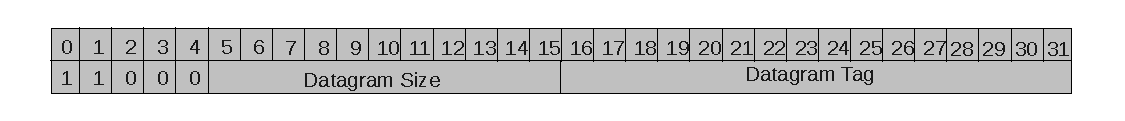
\includegraphics[scale=0.8]{/home/bo/Documents/Miniproject/Pics/Fragmentation_1.pdf}}\\
    \subfloat[Subsequence fragmentation]{\label{fig:Fragmentation_2}
       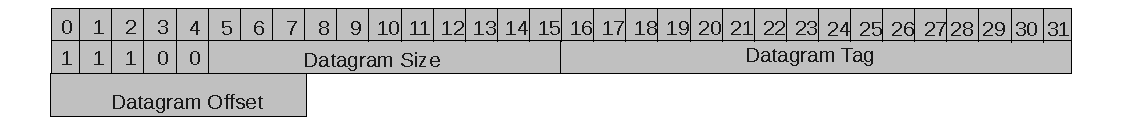
\includegraphics[scale=0.8]{/home/bo/Documents/Miniproject/Pics/Fragmentation_2.pdf}}
    \caption{Fragmentation header of 6LoWPAN}
    \label{fig:Fragmentation}
  \end{center}
\end{figure}
\index{figure 1.2}
\vspace{-10pt}
\begin{figure}[htbp]
  \begin{center}
    \leavevmode
    %\framebox{
      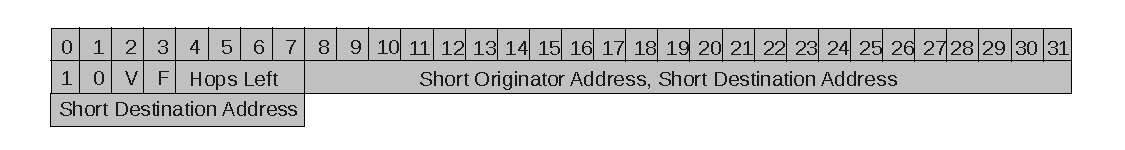
\includegraphics[scale=0.8]
      {/home/bo/Documents/Miniproject/Pics/Mesh.pdf}%}
    \caption{Mesh addressing header of 6LoWPAN}
    \label{fig:Mesh}
  \end{center}
\end{figure}
\index{figure 1.2}

The protocol stack of an LBR is given in  Figure~\ref{fig:LBR}. It is a network layer router; when packets are routed though the LBR to an external IPv6 based network, the adaptation
layer in the LBR translates the LoWPAN format header into a full IPv6 format, and
vice versa. In some practical applications, the adaptation layer is implemented along with an IP
layer such as, for example, in BLIP on the WSN nodes.
\vspace{7pt}
\begin{figure}[htbp]
  \begin{center}
    \leavevmode
   % \framebox
    \caption{LBR protocol stack}
    \label{fig:LBR}
    \vspace{-10pt}
  \end{center}
\end{figure}
%\index{figure 1.1}

\section{An Implementation of 6LoWPAN}
\label{Intr:Implementation}

There are several implementations for 6LoWPAN, such as uIPv6, BLIP, Sensinode's NanoStack, Jennic's 6LoWPAN and Nivis ISA100~\cite{ShelbyBormann2009}. The first two are open-source protocol stacks
for embedded operating systems, Contiki and TinyOS. The latter are commercial protocol stacks. 

\subsection{BLIP}
\label{Intr:BLIP}
BLIP, which stands for the Berkeley Low-power IP stack, is an implementation of 6LoWPAN in
TinyOS. TinyOS is a light-weight open source operating system which runs on sensor nodes in
WSNs. It allows for various applications to be installed on sensor nodes via USB connections.
\newline

The programming language used in TinyOS is called NesC - a dialect of the C language. It is
a component-based as well as event-driven programming language; the components are wired
together using interfaces. These features make the operating system optimized for the memory constraints of sensors. The supported hardware platforms for TinyOS include: Mica,
Mica2, and TelosB. Using BLIP/TinyOS, one is able to form multi-hop IP networks
consisting of different motes~\cite{BLIP}. 
\newline

BLIP contains both UDP and TCP protocols, as well as several application protocols. One standard network testing application, UDPEcho, is used in this mini project to verify the quality of the network. Another application, IPBaseStation, is installed in a sensor node which is connected to an embedded Linux device via USB connection.  This sensor node along with the embedded Linux device will together act as an LBR.
\newline

The next chapter will focus on the simulation of BLIP implemented WSN.


%}}}

%{{{ Emacs Local Variables

% Local Variables: 
% mode: latex
% TeX-master: "studentprojectthesis"
% TeX-command-list: (("TeX" "tex '\\nonstopmode\\input %t'" TeX-run-TeX nil t) ("TeX Interactive" "tex %t" TeX-run-interactive nil t) ("LaTeX" "%l '\\nonstopmode\\input{%t}'" TeX-run-LaTeX nil t) ("LaTeX Interactive" "%l %t" TeX-run-interactive nil t) ("LaTeX2e" "latex2e '\\nonstopmode\\input{%t}'" TeX-run-LaTeX nil t) ("SliTeX" "slitex '\\nonstopmode\\input{%t}'" TeX-run-LaTeX nil t) ("View" "%v " TeX-run-background t nil) ("Print" "%p " TeX-run-command t nil) ("Queue" "%q" TeX-run-background nil nil) ("File" "dvips %d -o %f " TeX-run-command t nil) ("BibTeX" "bibtex %s" TeX-run-BibTeX nil nil) ("Index" "makeindex -s indexeng.ist %s" TeX-run-command nil t) ("Check" "lacheck %s" TeX-run-compile nil t) ("Spell" "<ignored>" TeX-run-ispell nil nil) ("Other" "" TeX-run-command t t) ("Makeinfo" "makeinfo %t" TeX-run-compile nil t) ("AmSTeX" "amstex '\\nonstopmode\\input %t'" TeX-run-TeX nil t) ("GloTeX" "glotex %t" TeX-run-command nil nil))
% folded-file: t
% End: 

%}}}
